% !TEX TS-program = pdflatex
% !TEX encoding = UTF-8 Unicode

% This file is a template using the "beamer" package to create slides for a talk or presentation
% - Giving a talk on some subject.
% - The talk is between 15min and 45min long.
% - Style is ornate.

% MODIFIED by Jonathan Kew, 2008-07-06
% The header comments and encoding in this file were modified for inclusion with TeXworks.
% The content is otherwise unchanged from the original distributed with the beamer package.

\documentclass{beamer}


% Copyright 2004 by Till Tantau <tantau@users.sourceforge.net>.
%
% In principle, this file can be redistributed and/or modified under
% the terms of the GNU Public License, version 2.
%
% However, this file is supposed to be a template to be modified
% for your own needs. For this reason, if you use this file as a
% template and not specifically distribute it as part of a another
% package/program, I grant the extra permission to freely copy and
% modify this file as you see fit and even to delete this copyright
% notice. 


\mode<presentation>
{
  \usetheme{default}
  % or ...

  \setbeamercovered{transparent}
  % or whatever (possibly just delete it)
}


\usepackage[english]{babel}
% or whatever

\usepackage[utf8]{inputenc}
% or whatever

\usepackage{times}
\usepackage[T1]{fontenc}
\RequirePackage[numbers,sort&compress,square,comma]{natbib}
\bibliographystyle{IEEEtranN}
% Or whatever. Note that the encoding and the font should match. If T1
% does not look nice, try deleting the line with the fontenc.


\title[Parallel Graph Reduction] % (optional, use only with long paper titles)
{Easy parallel functional programming, the hard way.}

\subtitle
{} % (optional)

\author[] % (optional, use only with lots of authors)
{J. M. Calderon Trilla}
% - Use the \inst{?} command only if the authors have different
%   affiliation.

\institute[University of York] % (optional, but mostly needed)
{%
  Department of Computer Science\\
  PLASMA Research Group \\
  University of York
 }
% - Use the \inst command only if there are several affiliations.
% - Keep it simple, no one is interested in your street address.

\date[] % (optional)
{19-01-2012 / Literature Review Seminar}

\subject{Talks}
% This is only inserted into the PDF information catalog. Can be left
% out. 



% If you have a file called "university-logo-filename.xxx", where xxx
% is a graphic format that can be processed by latex or pdflatex,
% resp., then you can add a logo as follows:

% \pgfdeclareimage[height=0.5cm]{university-logo}{university-logo-filename}
% \logo{\pgfuseimage{university-logo}}



% Delete this, if you do not want the table of contents to pop up at
% the beginning of each subsection:
\AtBeginSubsection[]
{
  \begin{frame}<beamer>{Outline}
    \tableofcontents[currentsection,currentsubsection]
  \end{frame}
}


% If you wish to uncover everything in a step-wise fashion, uncomment
% the following command: 

%\beamerdefaultoverlayspecification{<+->}


\begin{document}

\begin{frame}
  \titlepage
\end{frame}

\begin{frame}{Outline}
  \tableofcontents
  % You might wish to add the option [pausesections]
\end{frame}


% Since this a solution template for a generic talk, very little can
% be said about how it should be structured. However, the talk length
% of between 15min and 45min and the theme suggest that you stick to
% the following rules:  

% - Exactly two or three sections (other than the summary).
% - At *most* three subsections per section.
% - Talk about 30s to 2min per frame. So there should be between about
%   15 and 30 frames, all told.

\section{Introduction}

\subsection[Motivation]{Motivation}

\begin{frame}{Why Functional Programming?}
    \begin{itemize}
        \item
            Parallel programming in imperative style is difficult. The lack of state in
            functional programs provides an advantage \cite{PFPAnIntro}.
        \item
            The largest successes in large scale parallelism have come from the declarative
            and functional paradigms (Databases, Map/Reduce).
    \end{itemize}
\end{frame}

\begin{frame}{What's taken to long?}
    \begin{itemize}
        \item
            Throughout the 80's researchers worked on parallel graph reduction for functional
            programs. However, the research could not keep up with the massive increase
            in single CPU processing speed/power. 
        \item
            Moore's law is still holding, but single thread CPUs are not seeing the same speed
            increases. Additional power is continually coming from increasing the number of 
            processing cores.
             
    \end{itemize}
\end{frame}

\subsection[Research Popularity]{Research Popularity}

\begin{frame}[fragile]{Popularity of Parallel Functional Programming}{}
    \begin{figure}
    \centering
        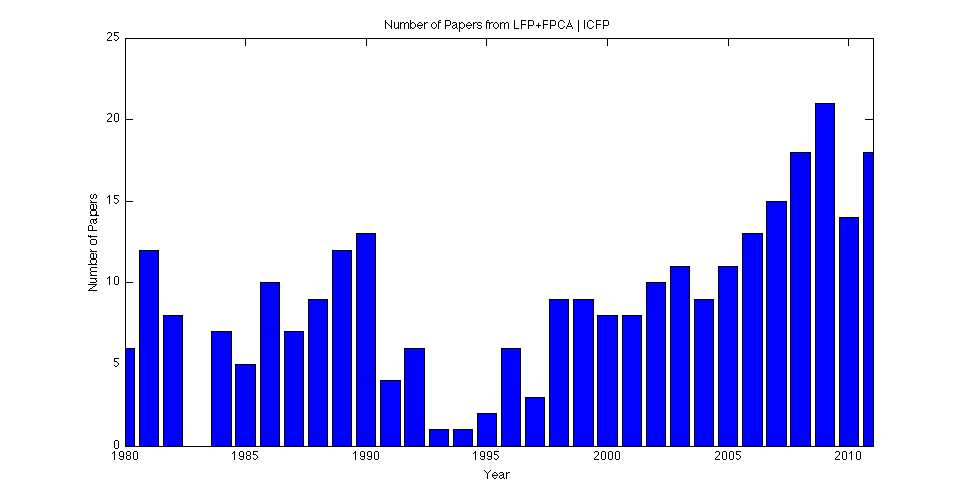
\includegraphics[scale=.4]{figures/numPapers.png}
        \caption{The ebb and flow of PFP}
    \end{figure}

\end{frame}

\section{Abstract Machines}

\begin{frame}{General Properties}
\end{frame}

\subsection[The $< \nu, G> Machine$]{The $< \nu, G> Machine$}

\begin{frame}{Simple G-Machine}
Stack based machine with `G-Code' used as an intermediate language. G-Code is generated for
every supercombinator in the program, leaving the G-Machine with a set of G-Code fragments.  
    \begin{figure}
    \centering
        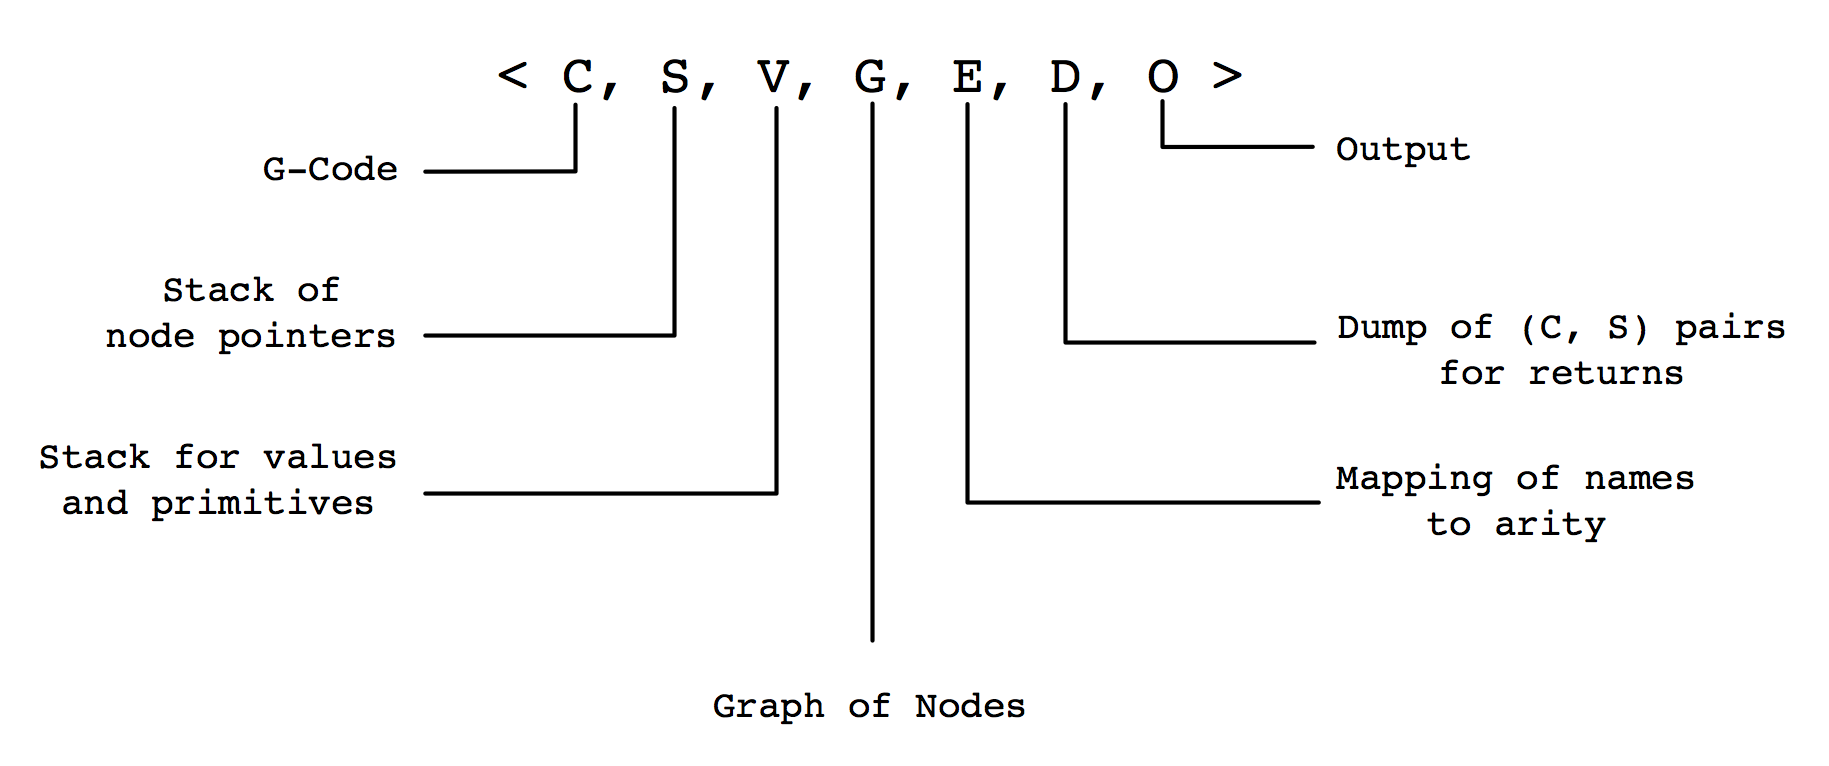
\includegraphics[scale=.3]{figures/GMachineState.png}
    \end{figure}
\end{frame}

\begin{frame}{Example Graph Reduction}
    \begin{figure}
    \centering
        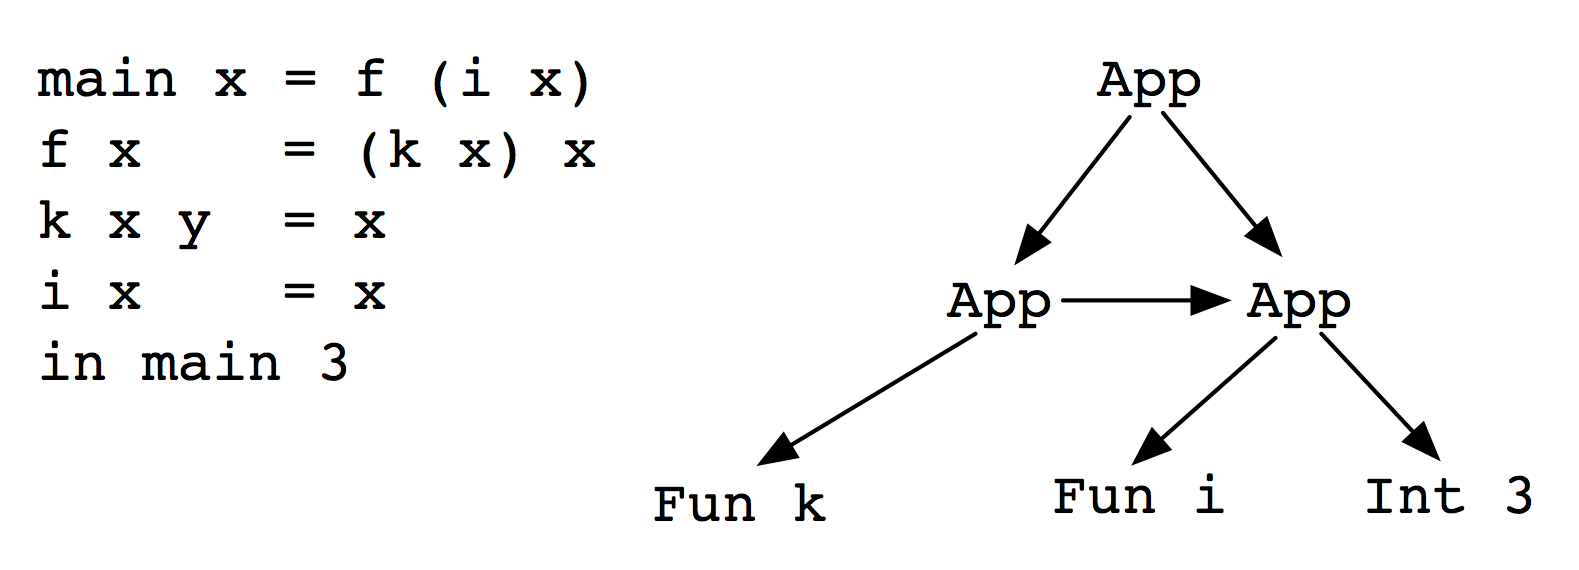
\includegraphics[scale=.3]{figures/GraphRed1.png}
    \end{figure}
\end{frame}

\begin{frame}{Simple Parallelization}
    \begin{figure}
    \centering
        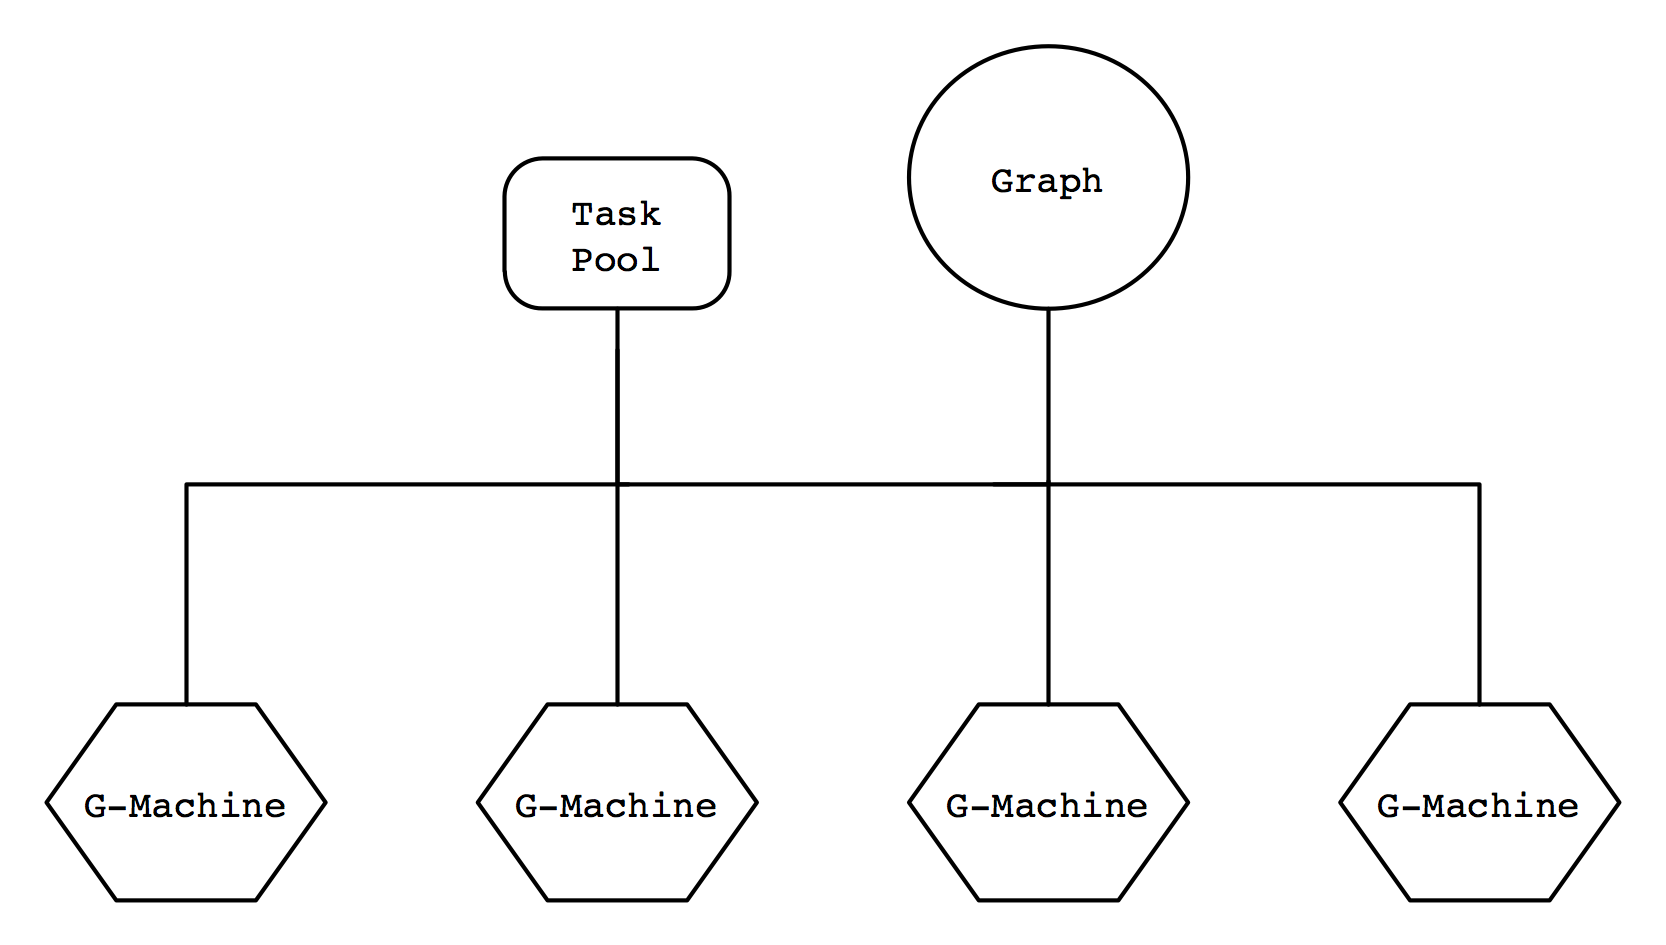
\includegraphics[scale=.3]{figures/simpleParallel.png}
    \end{figure}
\end{frame}

\begin{frame}{$<\nu, G> Machine$}
Packet based, shares task and graph
\end{frame}


\subsection[The ABC Machines]{The ABC Machine}
\begin{frame}{Basics}
Packet based, shares task and graph
\end{frame}

\section{Physical Machines}

\subsection[GRIP]{GRIP: Graph Reduction In Parallel}
\begin{frame}[fragile]{What GRIP looks like}{}

\begin{figure}[h]
 \centering
 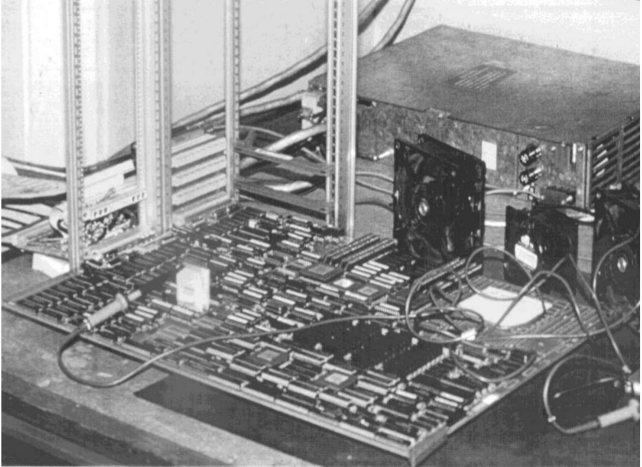
\includegraphics[scale=.4]{figures/GRIP.png}
 \caption{A circuit board for the GRIP machine in the making \cite{PFPAnIntro}}
\end{figure}
\end{frame}

\subsection[ALICE]{ALICE}

\begin{frame}{Quantum Dots as Artificial Atoms}{}
  % - A title should summarize the slide in an understandable fashion
  %   for anyone how does not follow everything on the slide itself.

  Quantum Confinement in 3D -> Artificial atom
  \begin{itemize}
  \item
   Question: What atomic properties are we looking to exploit?
   \pause
  \item
    Answer: Fluorescence.
  \end{itemize}
\end{frame}


\section*{Questions}

\begin{frame}
\centering
Questions
\end{frame}
\begin{frame}
\bibliography{seminar}

\end{frame}
\end{document}


